%%%%%%%%%%%%%%%%%%%%%%%%%%%%%%%%%%%%%%%%%
% FRI Data Science_report LaTeX Template
% Version 1.0 (28/1/2020)
% 
% Jure Demšar (jure.demsar@fri.uni-lj.si)
%
% Based on MicromouseSymp article template by:
% Mathias Legrand (legrand.mathias@gmail.com) 
% With extensive modifications by:
% Antonio Valente (antonio.luis.valente@gmail.com)
%
% License:
% CC BY-NC-SA 3.0 (http://creativecommons.org/licenses/by-nc-sa/3.0/)
%
%%%%%%%%%%%%%%%%%%%%%%%%%%%%%%%%%%%%%%%%%


%----------------------------------------------------------------------------------------
%	PACKAGES AND OTHER DOCUMENT CONFIGURATIONS
%----------------------------------------------------------------------------------------
\documentclass[fleqn,moreauthors,10pt]{ds_report}
\usepackage[english]{babel}
\usepackage{tcolorbox}
\usepackage{etoolbox}
\usepackage{todonotes}
\usepackage{numprint}
\usepackage{float}
\usepackage{cleveref}

\setuptodonotes{inline,backgroundcolor=yellow}

\graphicspath{{fig/}}




%----------------------------------------------------------------------------------------
%	ARTICLE INFORMATION
%----------------------------------------------------------------------------------------

% Header
\JournalInfo{FRI Natural language processing course 2024}

% Interim or final report
\Archive{Project report} 
%\Archive{Final report} 

% Article title
\PaperTitle{\textcolor{red}{WIP}: Literary Conversational Agents}

% Authors (student competitors) and their info
\Authors{Žiga Trček, Matej Urbas, and Jan Vasiljević}

% Advisors
\affiliation{\textit{Advisors: Slavko Žitnik}}

% Keywords
\Keywords{\textcolor{red}{DRAFT}, conversational agents, large language models, in-context-learning}
\newcommand{\keywordname}{Keywords}


%----------------------------------------------------------------------------------------
%	ABSTRACT
%----------------------------------------------------------------------------------------

\Abstract{
\textcolor{red}{DRAFT:} Engaging audiences deeply with literature is crucial for enhancing global literacy levels. In this study, we build upon the foundation of conversational agents, which have historically underperformed but have recently been revolutionized by advancements in large-scale language models. We fine-tune various foundational models and assess their enhanced capabilities using a series of standardized quizzes that we introduce. Our focus is on popular literary series, specifically "A Song of Ice and Fire" and "Harry Potter." Additionally, we underscore the significance of employing In-Context Learning to effectively emulate the dialogue styles of key characters within these series, thereby enriching the interactive reading experience.
}

%----------------------------------------------------------------------------------------

\begin{document}

% Makes all text pages the same height
\flushbottom

% Print the title and abstract box
\maketitle

% Removes page numbering from the first page
\thispagestyle{empty}

%----------------------------------------------------------------------------------------
%	ARTICLE CONTENTS
%----------------------------------------------------------------------------------------

\section*{Introduction}

Literacy among young people is declining, as highlighted in \cite{murray2021literacy}. Many young people have a disinterest in reading and seldom read for enjoyment. A potential strategy to encourage reading is to involve them in conversational interactions with digital pedagogical agents that imitate well-known literary figures. Although numerous studies, such as those \cite{nielen2018digital,alaimi2020pedagogical}, discuss the advantages of pedagogical agents, detailed technical implementation aspects are often overlooked. Our work aims to explore various methods for creating pedagogical agents and to provide a comprehensive technical implementation for the method we choose.

\subsection*{Related work}
Setting and situational continuity are important for user experience. \cite{situation_models} conducted experiments showing that discontinuities in time, space, causation, motivation, and protagonist dimensions increase reading time, supporting the "processing-load hypothesis."

Educational agents benefit from effective teaching strategies. An analysis of Dutch reading comprehension textbooks \cite{bogaerds2022textbooks} found a lack of alignment between lesson goals, theory, and assignments. Teaching all three knowledge types — declarative, procedural, and conditional — could improve literacy.

Social bots capable of engaging in open-domain conversations, like Alana \cite{papaioannou2022designing}, require maintaining context, providing coherent responses, and being engaging and knowledgeable. Alana achieves this through an ensemble of specialized bots, with a ranker determining the best response, and a state object storing previous conversation information.

Retrieval-augmented generation (RAG) is used to correct factually inaccurate or outdated LLM outputs. A survey by \cite{gao2023retrieval} categorizes RAG methods into pre-training, fine-tuning, and inference, with inference being the most common today. FLARE \cite{jiang2023active} re-prompts the LLM with additional data for low-probability tokens.

Training or fine-tuning LLMs to create agents is demonstrated by \cite{shao2023characterllm}, which developed conversational agents resembling historical figures using Experience Reconstruction, Protective Experience, and Experience Upload techniques.

Data augmentation for character training is addressed by PEDANT \cite{neuman2023data}, which generates data using a GPT model combined with domain expertise. This approach was validated using text classification tasks on offensive-speech datasets.

To avoid training a LLM, prompt engineering, specifically Chain-of-Thought (COT), can be used \cite{jeong2023chatbot}. Employing Information-Rich Prompts (IRP) that include emotional state, relationship context, and memories, enhances responses. Incorporating the Big Five personality model \cite{goldberg1990thebigfive} could further refine responses.

BookNLP \cite{booknlp}, an NLP pipeline for analyzing literary texts, performs POS tagging, dependency parsing, entity recognition, co-reference resolution, and more. Built on SpaCy \cite{spacy2} and using BERT \cite{joshi2019bert}, it effectively extracts and attributes dialogues to characters.
%------------------------------------------------

\section*{Methods}

\begin{figure*}[htp]
	\centering
	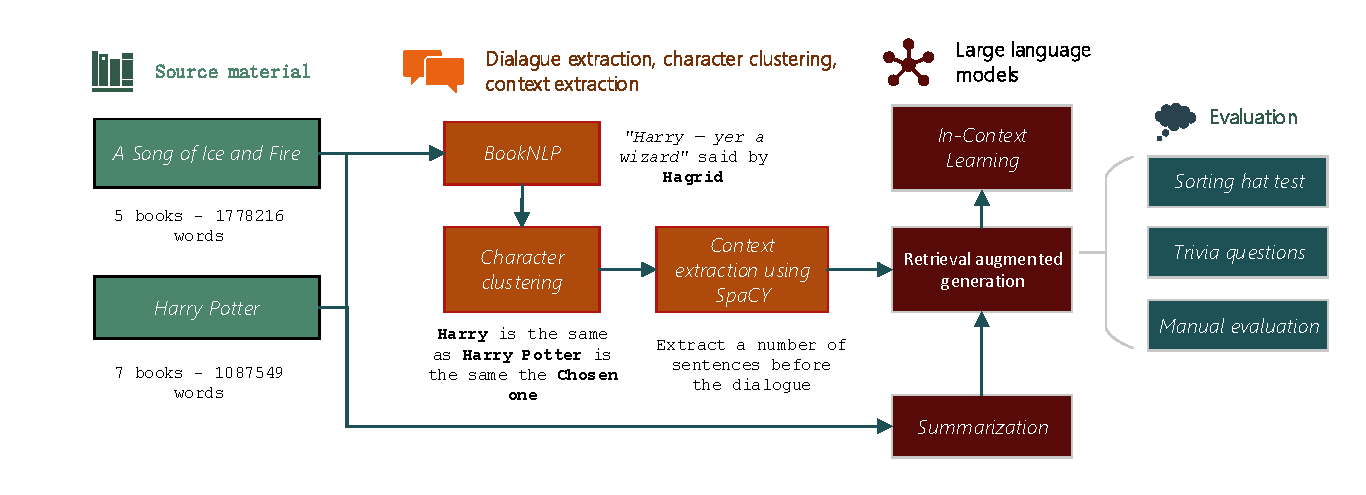
\includegraphics[width=\linewidth]{pipeline.pdf}
	\caption{\textbf{Our proposed pipeline.} High-level overview of our pipeline and methods used in the final project.}
	\label{fig:pipeline}
\end{figure*}

Our main approach to creating conversational agents revolves around data extraction from literary works. Based on this data, we provide the models with additional context to improve their performance. We tried several methods throughout the entire pipeline. However, based on numerous criteria, we settled on dialogue extraction, tagging characters from books, summarization, retrieval-augmented generation, and in-context learning. We will describe each of these steps in more detail.

As our source material, we chose two popular book series: \textit{A Song of Ice and Fire} (ASoIaF) \cite{book:asoiaf} by George R. R. Martin and \textit{Harry Potter} (HP) by J. K. Rowling \cite{book:hp}. ASoIaF comprises 5 books totaling \numprint{1778216} words, while HP consists of 7 books and \numprint{1087549} words. The two main reasons for this choice were the length of the books and the team's familiarity with the material. The books also differ significantly in style, providing a good test for our approaches.

\subsubsection*{Dialogue Extraction Using Instruct LLM}

We extracted all the dialogue along with the pre and post-context (10 sentences before and 2 sentences after each dialogue) and used Phi3 and Llama8B to classify the dialogue by identifying the speaker. We ignored dialogues shorter than 16 characters (as they were not meaningful) and longer than 500 characters (to save VRAM consumption). With a batch size of 10 dialogues, we classified all \numprint{40318} dialogues in 7 hours. We used a 2 and 4-shot prompt with examples of classification but did not achieve good results. There were three main reasons for this:

\begin{enumerate}
	\item The models did not possess good enough reasoning capabilities to classify the dialogues.
	\item Co-reference resolution was not adequate to classify the dialogues. When pronouns were used, the model did not know who was speaking most of the time.
	\item Information leakage: The models had some prior knowledge about the books, as they sometimes classified the dialogue with characters who were not even present in the pre or post-context or the dialogue itself.
\end{enumerate}

By validating the data by hand, we realized we would not achieve good enough results with this approach.

\subsubsection*{Dialogue Extraction Using BookNLP and Clustering}

We used BookNLP to extract dialogues from both books. The \texttt{big} model provided by the authors of BookNLP was utilized, which required 5-8 minutes of processing time per book. We also attempted to merge the books before processing to improve co-reference clustering and resolution; however, this resulted in memory segmentation faults, even on a machine with 128GB of RAM (Arnes). Consequently, we processed each book individually, necessitating the correct correlation (clustering) of character names across the series. This process involved normalizing names and removing duplicates by extracting sub-tokens and taking the root with the highest occurrence. If two sub-tokens had the same occurrence, we joined them, indicating a name with a space in it. For example, the character \textit{Hot Pie} from the series ASoIaF.

To validate the results, we manually reviewed randomly sampled dialogues. Based on this assessment, we assessed that approximately 90\% of the dialogues were correctly classified. Additionally, we constructed two graphs that show the dialogue frequency by character per book in the series (\cref{fig:asoif_dialogue} and \cref{fig:hp_dialogue}). Based on our familiarity with the books, we can confirm that the results are accurate. In the ASoIaF series, the chapters are also told from the perspective of the characters, so we matched the frequencies with their respective chapters. In total, we gathered \numprint{36946} dialogues from ASoIaF and \numprint{32541} from HP, totaling \numprint{69487} dialogues.

\begin{figure}[htb]
	\centering
	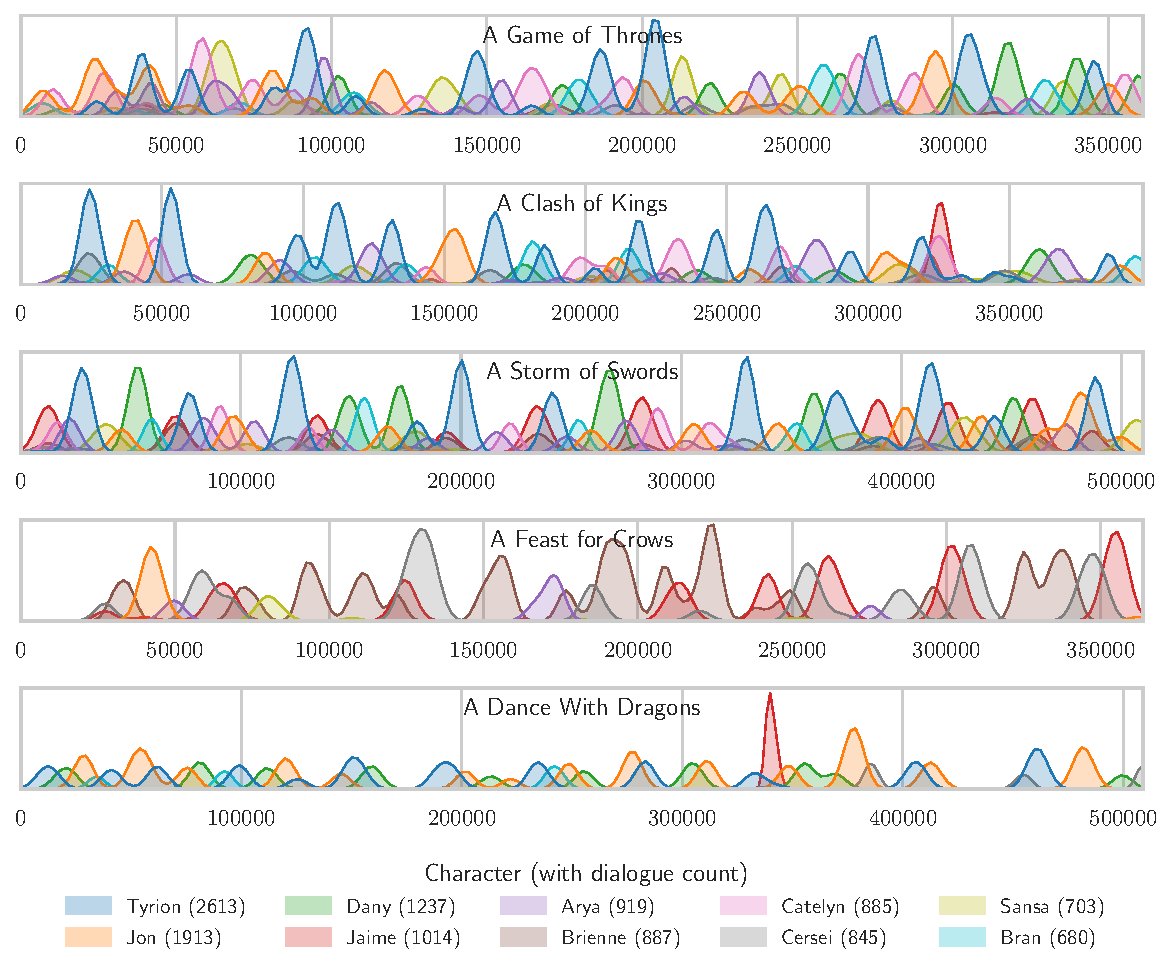
\includegraphics[width=\linewidth]{asoif_dialogue.pdf}
	\caption{\textbf{Dialogue from 10 most frequent characters in A Song of Ice and Fire.} This shows the dialogue frequency by character per book in the series. The x-axis represents the token count when the character speaks, while the y-axis is the kernel density estimate of the dialogue frequency.}
	\label{fig:asoif_dialogue}
\end{figure}


\begin{figure}[htb]
	\centering
	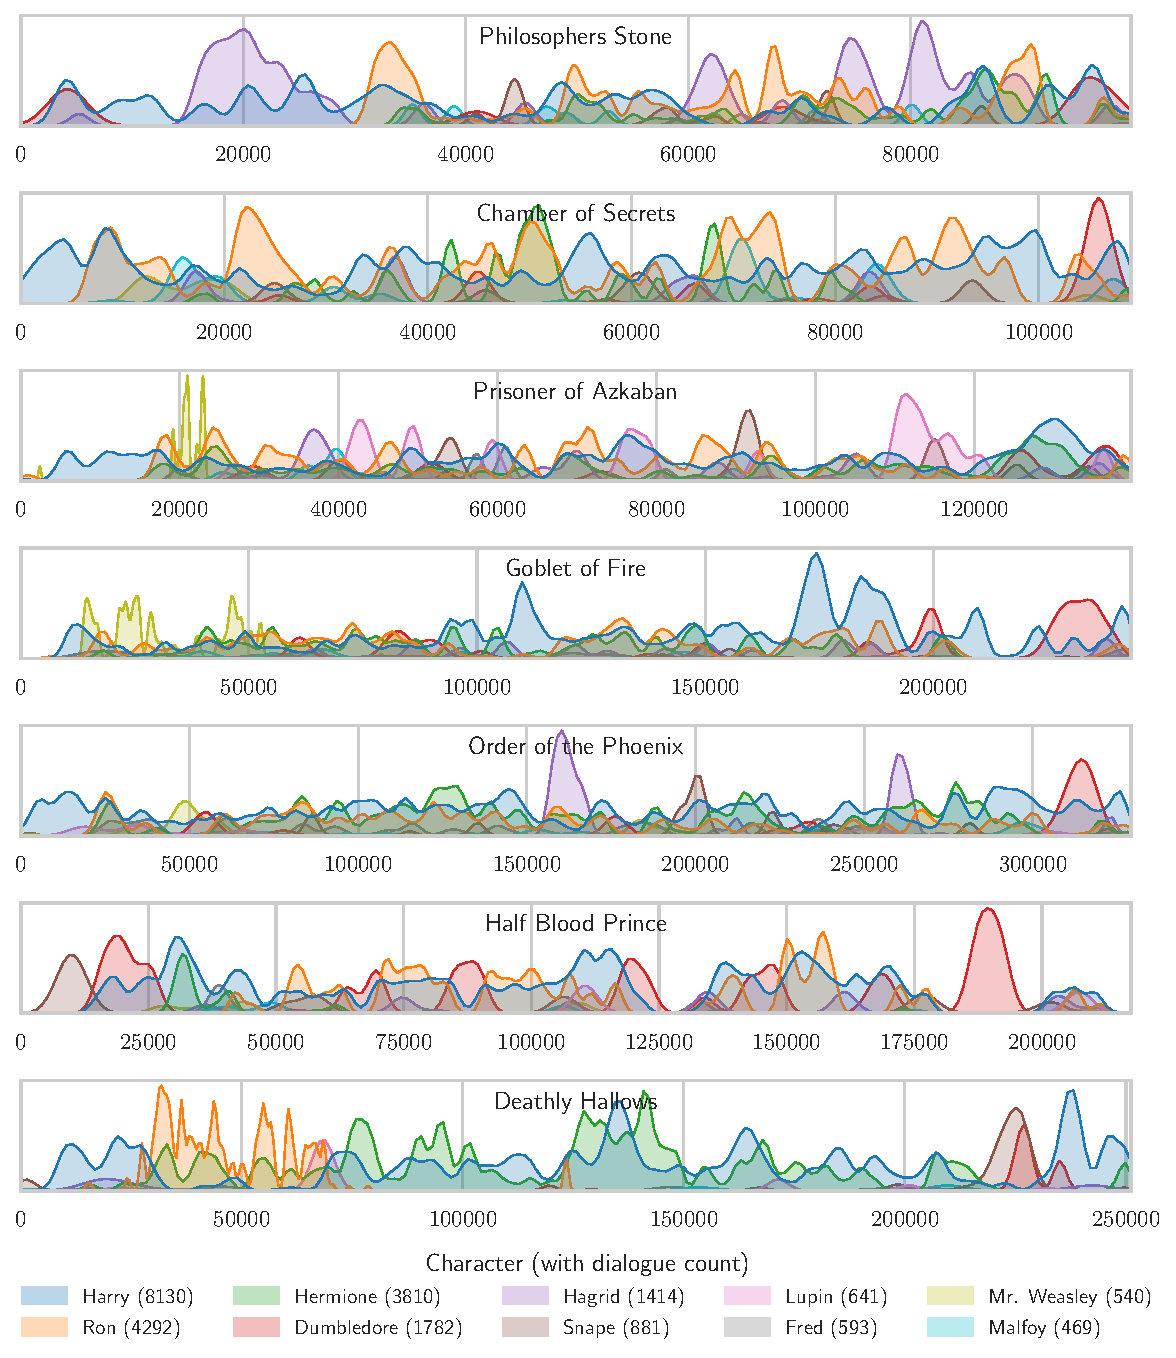
\includegraphics[width=\linewidth]{hp_dialogue.pdf}
	\caption{\textbf{Dialogue from 10 most frequent characters in the Harry Potter series.} This shows the dialogue frequency by character per book in the series. The x-axis represents the token count when the character speaks, while the y-axis is the kernel density estimate of the dialogue frequency.}
	\label{fig:hp_dialogue}
\end{figure}

\subsubsection*{Context extraction}

Before each dialogue, we extracted 3 chunks of 3 sentences each. We used the \textit{SpaCy} sentence tokenizer to split the text into sentences. With the constructed dataset, we gained the ability to selectively choose how much context to provide to the large language model (LLM) down the pipeline.

\subsubsection*{Other unsuscsessful attempts}

After extracting dialogues, we attempted several other methods to extract data from the books. The goal was to enhance the conversational model by providing it with more context from the books. These methods included:

\begin{enumerate}
	\item Extracting factual information from the books by re-using named entity recognition (NER) entities related to the characters. We extracted subject-verb-object triples from the books to gain more information about the characters. However, due to the complexity of the language used in the books, the extraction did not yield meaningful results.

	\item Recursively summarizing the character behaviors to achieve a better understanding of their personalities and relationships. We used Phi3 with a 128k context window to recursively summarize sections of the books that included a particular character of interest. This approach, however, did not succeed. It was computationally expensive (even after splitting into 20k chunks, the model used upwards of 60GB of graphics memory) and the results were inadequate. Despite claims that the model can handle tasks within a long context, the results showed that the model completely forgot the instructions after utilizing only one-eighth of its theoretical context window.

	\item Using DistilBART for question answering. Our final attempt was to extract key information about characters from the books (such as character locations, ages, etc.) and use DistilBART to answer questions. This was intended to serve as in-context learning for our conversational agents. However, this approach also failed due to the complex language used in the books.

	\item While not entirely related to dialogue extraction, our first attempt at the problem included fine-tuning Phi 3 and Llama 8B on the \textit{Harry Potter} series. We used a chunk size of 512 characters with an overlap of 64 characters. The models were trained on overlapping chunks of text to ensure that they learned the context of the conversation. However, it was evident by the end of the training that the models did not learn much. The source material was already included in the pretraining data of the models, so the fine-tuning did not provide any significant improvements.

\end{enumerate}

\subsection*{Book summaries}

The characters' dialogues can give the language model an idea of how a specific character speaks; however, it can still use more context to formulate better answers. Furthermore, much of the important contextual information cannot be extracted from speech alone. By providing the language model with extra content from the books, we hoped to increase its performance in some evaluation tasks.

Original texts are quite long. ASoIaF consists of around 1.7 million words, while the HP series is a bit shorter, with 1.1 million words. Therefore, we split the books into smaller chunks and summarized each of them. We tried a few different summarization language models from HuggingFace. These included
\texttt{bart-large-cnn} \cite{bart_large}, \texttt{google-t5/t5-large} \cite{2020t5}, \texttt{google/pegasus-xsum} \cite{zhang2019pegasus} and \texttt{Falconsai/\-text\_summarization}.

By examining the outputs, we concluded that Falconsai's model provided the best summarizations. It has a context window of \numprint{512}  tokens; therefore, we split the books into chunks smaller than \numprint{512} tokens. Splitting was done only between sentences, so they were never cut in half, which resulted in chunks being smaller than \numprint{512} tokens.

This gave us \numprint{6275} chunks from ASoIaF and \numprint{4716} chunks from the HP series. Summarizing all \numprint{10991} chunks took about 6 hours and resulted in approximately a six-fold reduction in word count. The summarized ASoIaF consists of around 300k words and the summarized HP series consists of around 200k words.

\subsection*{Retrieval-Augmented Generation}

We stored the selected characters' dialogues, with or without surrounding context, in a FAISS vector database. During inference, the database was queried by the user's question and returned between 10 and 30 promising character lines, which were then used to create the model prompt. The same process was applied to book summaries to provide the model with additional context.

\subsection*{In-Context Learning}

The closest retrieved dialogues, summaries, and other contexts were included in the prompt to provide the model with more context. This was done to improve the model's performance on the quiz questions and to make it more engaging in dialogue.

%------------------------------------------------

\section*{Results}
Most of the evaluation was manual, therefore slightly subjective.
It was done independently by all three team members and averaged into the final conclusion.

\subsection*{Character evaluation}

\begin{figure*}[hbt]
	\centering
	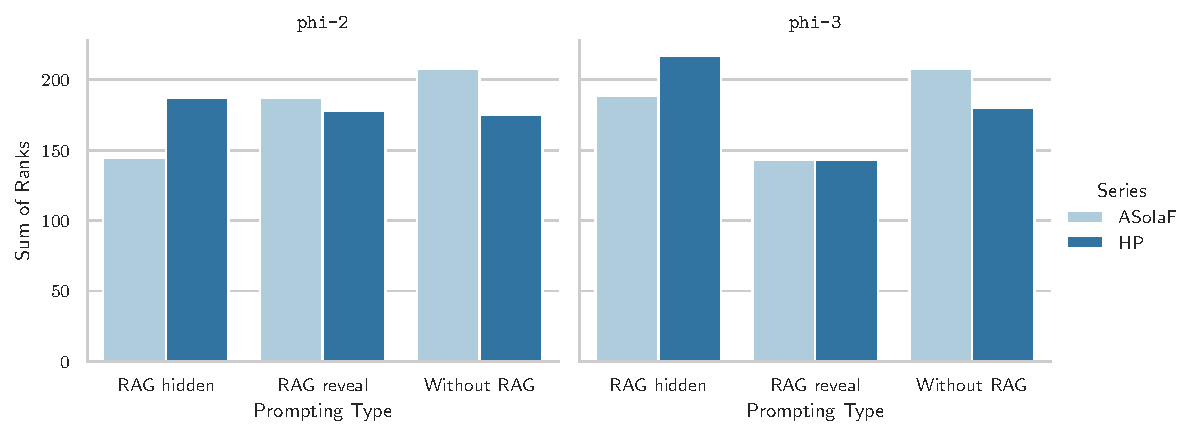
\includegraphics[width=0.8\linewidth]{questioners-results.pdf}
	\caption{\textbf{Evaluation}: Sum of ranks for both models and all three prompting strategies. Lower is better.}
	\label{fig:character_evaluation_results}
\end{figure*}


We looked at the language model's ability to speak as a selected character.
For this test we picked 6 characters, 3 from both series.
From the Harry Potter franchise we picked Harry Potter himself, headmaster Dumbledore and antagonist Voldemort.
For A Song of Ice and Fire we picked mother of dragons Daenerys, lord commander John Snow and the best door holder Hodor.

We created a list of questions for every character.
There are 8 non-specific questions (for all 6 characters), 9 Harry Potter specific questions, 14 ASOIF specific questions
and for each character an additional 4-8 questions.
In total there are 30 different questions for Harry Potter and 40 questions for ASOIF characters.

The biggest evaluation problem was quite unexpected. It was very difficult to find an appropriate large language model for this task.
Bigger language models, such as Llama-3-8B \cite{llama3modelcard} or Mistral-7B \cite{jiang2023mistral} were already so familiarized with both series that the model worked good without any modifications.
Smaller language models, such as TinyLlama-1.1B \cite{zhang2024tinyllama}, GPT2 \cite{radford2019language} or Google Gemma-2B \cite{gemma_2024},
were either unable to act as a given character (saying that they are a langauge model and unable to answer the question)
or their answers were very random, and not connected to the books in any way, despite trying several different prompts and RAG strategies.
In the end we decided to use Microsoft's Phi-3 \cite{abdin2024phi} and Phi-2 models, pretrained for instruction tasks.
These two models weren't as familiar with the characters but were still able to somewhat act as the desired character.

For each character we tested three different prompting strategies:
\begin{itemize}
	\item Prompt contained only the name of the character and the book series and some instructions how to act. This was done so that we can get a rough baseline of what the model knows and how it behaves out of the box.
	\item RAG reveal: This prompt extended the previous one with dialogues and other context retrieved from the vector database.
	\item RAG hidden: This prompt didn't state the character name or the book series. Only data that the model recieved was retireved from the vector database.
\end{itemize}

Each of the two models answered 150 questions across all characters using all three prompting strategies, which resulted in 900 total answers.
For every member in the group we randomly sampled 60 answers from Harry Potter and 60 from A Song of Ice and Fire.
Half of the questions were answered by Phi-2 and the other half with Phi-3.
Answers were randomly mixed, so that we didn't know which prompting strategy resulted in which answer.
We then ranked the answers from best to worst based on the overall structure, answer quality and information correctness.
In total we checked 360 questions with 1080 answers.
For each prompting strategy we summed its final ranks and sorted them accordingly.
Final rankings are shown in Figure \ref*{fig:character_evaluation_results}.

The best-performing model is Phi-3 with the RAG reveal strategy.
Other models and strategies are, however, more interesting to analyze.
If we exclude the best-performing model, we can observe that the strategies behave differently based on the chosen book series.
Performance of bots that emulate ASoIaF's characters increases when we first add RAG and then increases again when we remove the character name and series from the prompt.
However, with Harry Potter's characters, we can see a slight decrease in performance when adding RAG and then another decrease when removing the name and series information.
There is a chance that this happened because of our manual, subjective evaluation.
However, when we examined the dialogues from both series, we found that the dialogues in ASoIaF are much longer and contain more useful information.
Dialogues from Harry Potter are shorter and often lack meaningful information.

\subsection*{Sorting hat test}
We thought it would be interesting to evaluate our Harry Potter characters with the sorting hat test.
This evaluation was done out of curiosity. The rules and questions of the sorting test are not really stated inside the books.
We scraped a random online sorting hat quiz which looked promising and easy to use.
We used the quiz on 8 different characters, 2 from each house:
\begin{itemize}
	\item Gryffindor: Harry and Dumbledore,
	\item Slytherin: Snape and Draco,
	\item Ravenclaw: Cho and Luna,
	\item Hufflepuff: Cedric and Tonks.
\end{itemize}
Each character was tested with all three prompting strategies, with Phi-3 as the language model.
We ran the test 10 times for every character.
The test results are shown in Table \ref*{tab:sorting_hat_results}.
Correct house predictions are in bold, number in parantheses is the number of times this house was selected among all 10 tries.

\begin{table}[hbt]
	\caption{Sorting hat results}
	\centering
	\begin{tabular}{c | c | c | c }
		Character  & Without RAG         & RAG hidden         & RAG reveal          \\ \hline
		Harry      & Raven (5)           & \textbf{Gryff (9)} & \textbf{Gryff (6)}  \\
		Dumbledore & Raven (7)           & \textbf{Gryff (7)} & Raven (7)           \\ \hline
		Snape      & \textbf{Slyth (10)} & Gryff (7)          & Gryff (7)           \\
		Draco      & \textbf{Slyth (10)} & Gryff (7)          & \textbf{Slyth (10)} \\ \hline
		Cho        & \textbf{Raven (7)}  & Gryff (6)          & \textbf{Raven (9)}  \\
		Luna       & \textbf{Raven (6)}  & Gryff (9)          & \textbf{Raven (8)}  \\ \hline
		Cedric     & Slyth (10)          & Raven (5)          & Raven (6)           \\
		Tonks      & Gryff (9)           & Gryff (5)          & Gryff (10)          \\
	\end{tabular}
	\label{tab:sorting_hat_results}
\end{table}

As expected, this test didn't bring any meaningful results.
When the character is hidden from the model, it almost always predicts Gryffindor, which makes the correct guess for Harry and Dumbledore meaningless.
When character is revealed to the model, it correctly sorts half of the characters. RAG doesn't really effect the outcome of the sort.
We can therefore assume, that the quotes and context from RAG are not really useful for this test.
We tried to run the test on Llama-3-8B, which should have deeper understanding of characters out of the box to see how it performs.
Results are shown in Table \ref*{tab:sorting_hat_results_llama}.

\begin{table}[hbt]
	\caption{LLama-3 sorting hat results}
	\centering
	\begin{tabular}{c | c | c | c }
		Character  & Without RAG    & RAG hidden     & RAG reveal     \\ \hline
		Harry      & \textbf{Gryff} & \textbf{Gryff} & \textbf{Gryff} \\
		Dumbledore & Raven          & Raven          & Raven          \\ \hline
		Snape      & Raven          & Gryff          & Gryff          \\
		Draco      & Raven          & Gryff          & Gryff          \\ \hline
		Cho        & Gryff          & \textbf{Raven} & \textbf{Raven} \\
		Luna       & \textbf{Raven} & \textbf{Raven} & \textbf{Raven} \\ \hline
		Cedric     & Raven          & Gryf           & Raven          \\
		Tonks      & Gryff          & Raven          & Raven          \\
	\end{tabular}
	\label{tab:sorting_hat_results_llama}
\end{table}

These are even worse than with Phi-3. Here it only sorted the characters into Gryffindor and Ravenclaw.
We can conclude that this test is flawed in several ways: sorting questions are not stated in the books,
we can't really verify the validty of the used test
and questions in the quiz are often of philosophical/abstract nature which is not really interpretable by large langauge models.

%------------------------------------------------

\section*{Discussion}

The majority of our work was in extracting the dialogues from both book series.
This resulted in a big database of all dialogues from all 12 analysed books.
This database is still not perfect, there are some wrongly matched character-speech pairs.

%----------------------------------------------------------------------------------------
%	REFERENCE LIST
%----------------------------------------------------------------------------------------
\bibliographystyle{unsrt}
\bibliography{report}


\end{document}
